\section{Control}

\begin{figure}[h]
	\centering
	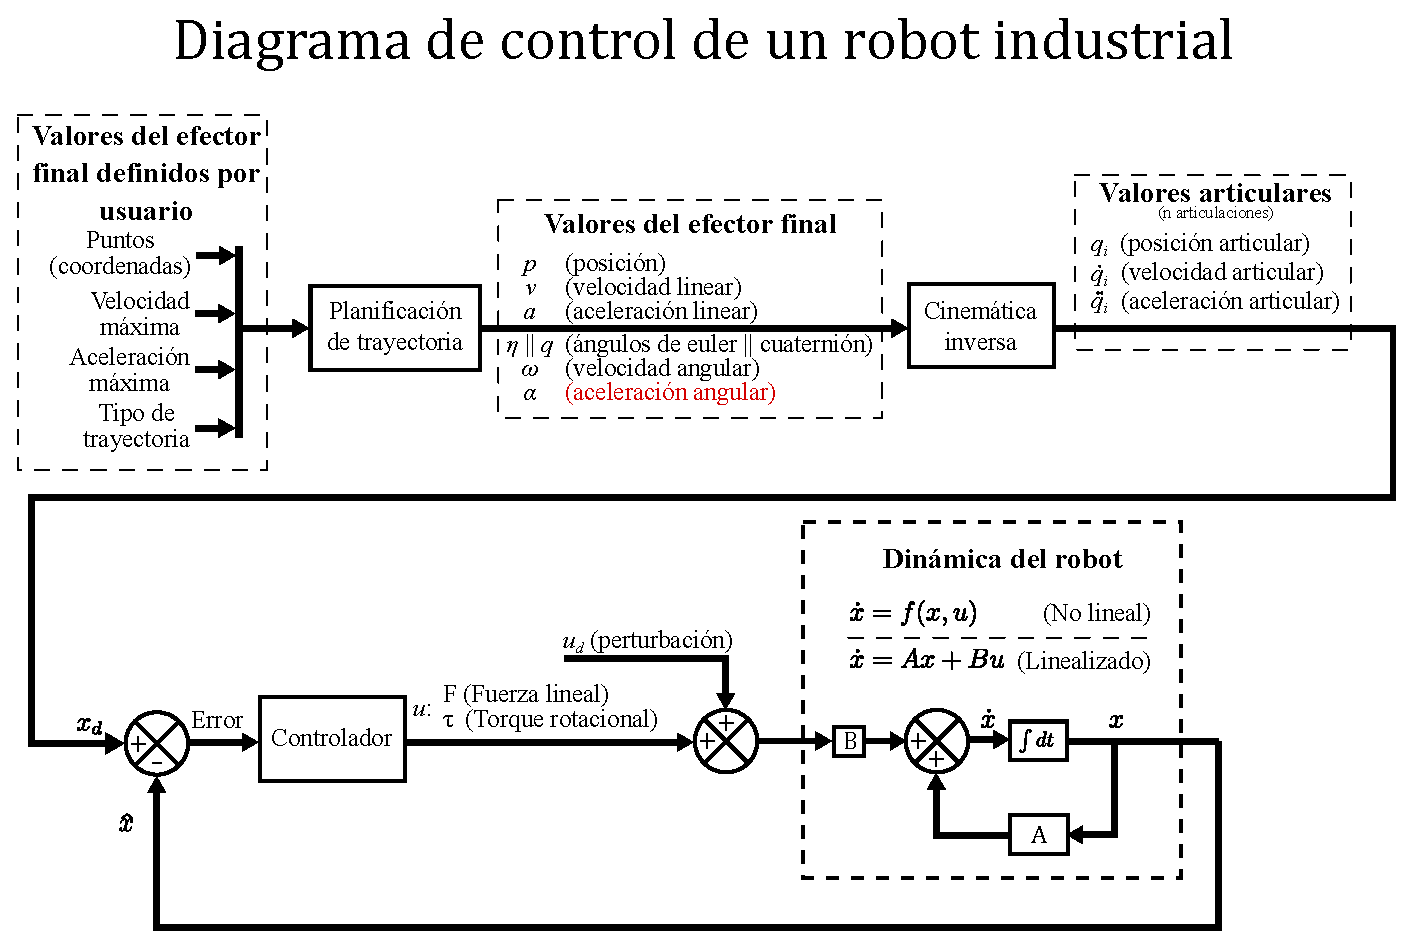
\includegraphics[width=\linewidth]{img/Diagrama_robot_industrial}
	\caption{Diagrama de bloques de un robot industrial}
	\label{fig:diagrama-de-robot-industrial}
\end{figure}

El diagrama de bloques de un robot industrial comienza con los valores del efector definidos por el usuario. Se ingresan datos como coordenadas de posición o destino final deseado del elemento como pinza o herramienta, velocidad máxima el cual es el límite de rapidez en la cual el elemento puede moverse, aceleración máxima y el tipo de trayectoria que realizará. 


Estos valores ingresan en la planificación de trayectoria donde se generan:\\[5pt]
-posición en el espacio cartesiano (x,y,z).\\[5pt]
-velocidad  lineal y angular.\\[5pt]
-aceleración lineal y angular.\\[5pt]
- |n| y q: orientación en ángulos de Euler.\\[5pt]


Posteriormente la cinemática inversa traduce los movimientos deseados a valores articulares que los motores deben ejecutar: \\[5pt]
-qi: posición articular\\[5pt]
-q’i: velocidad articular\\[5pt]
-q’’i: aceleración articular\\[5pt]


El siguiente bloque del diagrama es un controlador el cual compara el valor deseado de posición, velocidad y aceleración con el valor actual (el estado actual del elemento del robot). Se calcula el error y se genera una señal de control que puede ser de fuerza lineal o de torque rotacional. 


Posteriormente se entra a un controlador donde interactúan las perturbaciones externas o internas que pueden modificar el comportamiento del robot. 


Finalmente se llega al bloque de dinámica del robot el cual describe el comportamiento de las reacciones a las fuerzas o torques que se aplican. Dentro de esta sección se encuentran dos formas del modelo dinámico no lineal y linealizado. 
No lineal: Tiene en cuenta que las ecuaciones de movimiento dependen de la posición, velocidad y demás factores del robot. 
Linealizado: Es una aproximación para simplificar las ecuaciones no lineales y poderlas analizar y controlar más fácilmente. 

Dentro de este bloque se representa la integración numérica ya que a partir de la entrada de torque y posición inicial se calcula la aceleración, velocidad y posición de cada articulación y se actualiza el estado actual del robot en tiempo real. 

Después de cuenta con una retroalimentación para comparar con los valores deseados, se corrigen errores,  y nuevos cálculos de torques.

